\documentclass[bibtotoc,liststotoc,BCOR5mm,DIV12]{scrbook}

% use this declaration to set specific page margins
%\usepackage[a4paper , lmargin = {2.7cm} , rmargin = {2.9cm} , tmargin = {2.7cm} , bmargin = {4.6cm} ]{geometry}
\usepackage[a4paper]{geometry}

\usepackage[english]{babel}
%\usepackage{bibgerm}       		% german references
\usepackage[numbers,round]{natbib}
\usepackage[utf8]{inputenc} % german characters
\usepackage{graphicx} 				% it's recommended to use PDF images but you can use JPG or PNG as well
\usepackage{url}           		% format URLs
\usepackage{hyperref} 				% create hyperlinks
\usepackage{listings, color}	% for source code
\usepackage{subfig}						% two figures next to each other (example: figure 3a), figure 3b)
\usepackage{scrpage2}					% header and footer line
\usepackage{courier}
\usepackage{float}
\restylefloat{table}
\usepackage{tabularx} % in the preamble
%\usepackage{enumitem}
\usepackage{placeins}

% header and footer line - no header & footer line on pages where a new chapter starts
\pagestyle{scrheadings}
\ohead{LibChain}

\ihead{Cabello, Janßen, Mühle}
\ofoot[]{\thepage}
\ifoot{Project Report, TU Berlin, CIT, 2017}

% set path where images are stored
\graphicspath{{./img/}}

\definecolor{mygreen}{rgb}{0,0.6,0}
\definecolor{mygray}{rgb}{0.5,0.5,0.5}
\definecolor{mymauve}{rgb}{0.58,0,0.82}

\lstset{ %
  backgroundcolor=\color{white},   % choose the background color; you must add \usepackage{color} or \usepackage{xcolor}; should come as last argument
  basicstyle=\footnotesize,        % the size of the fonts that are used for the code
  breakatwhitespace=false,         % sets if automatic breaks should only happen at whitespace
  breaklines=true,                 % sets automatic line breaking
  captionpos=b,                    % sets the caption-position to bottom
  commentstyle=\color{mygreen},    % comment style
  deletekeywords={...},            % if you want to delete keywords from the given language
  escapeinside={\%*}{*)},          % if you want to add LaTeX within your code
  extendedchars=true,              % lets you use non-ASCII characters; for 8-bits encodings only, does not work with UTF-8
  frame=single,	                   % adds a frame around the code
  keepspaces=true,                 % keeps spaces in text, useful for keeping indentation of code (possibly needs columns=flexible)
  keywordstyle=\color{blue},       % keyword style
  language=Octave,                 % the language of the code
  morekeywords={*,...},           % if you want to add more keywords to the set
  numbers=left,                    % where to put the line-numbers; possible values are (none, left, right)
  numbersep=5pt,                   % how far the line-numbers are from the code
  numberstyle=\tiny\color{mygray}, % the style that is used for the line-numbers
  rulecolor=\color{black},         % if not set, the frame-color may be changed on line-breaks within not-black text (e.g. comments (green here))
  showspaces=false,                % show spaces everywhere adding particular underscores; it overrides 'showstringspaces'
  showstringspaces=false,          % underline spaces within strings only
  showtabs=false,                  % show tabs within strings adding particular underscores
  stepnumber=2,                    % the step between two line-numbers. If it's 1, each line will be numbered
  stringstyle=\color{mymauve},     % string literal style
  tabsize=2,	                   % sets default tabsize to 2 spaces
  title=\lstname                   % show the filename of files included with \lstinputlisting; also try caption instead of title
}

\lstset{
numbers=left,
breaklines=true,
captionpos=b,
showstringspaces=false,
basicstyle={\fontfamily{pcr}\selectfont\footnotesize}}


\lstset{numbers=left,breaklines=true,captionpos=b,showstringspaces=false,
basicstyle={\fontfamily{pcr}\selectfont\footnotesize}}
\newcommand{\imp}[1]{
\begin{center}
\colorbox{red}{{#1}}
\end{center}}

\newcommand{\impp}[1]{
(\colorbox{red}{{#1}})}

%
% der Befehl \hypenation versteht keine Sonderzeichen, also weder �
% noch "a noch \"a. W�rter die derartige Zeichen enthalten m�ssen
% direkt im Text getrennt werden, z.B. W�r\-ter
%
\hyphenation{te-le-com-muni-cation 
te-le-com-muni-cation-specific 
Te-le-kom-mu-ni-ka-tions-API} 					% use this file to set explicit hyphenations (doesn't seem to work correctly)

\begin{document}
% ---------------------------------------------------------------
\frontmatter
    \thispagestyle{empty}
\begin{center}
{\LARGE \textbf{Technische Universität Berlin}}

\vspace{0.5cm}

{\large CIT\\[1mm]}
{\large Complex and Distributed IT Systems\\[5mm]}

Faculty IV\\
Einsteinufer 17\\
10587 Berlin\\

\vspace*{1cm}

\includegraphics[width=5cm]{libchain_logo.jpg}
\vspace{0.6cm}

{\LARGE Project Report}\\
\vspace{0.3cm}
{\LARGE \textbf{LibChain - Open, Verifiable and Anonymous Access Management}}\\
\vspace*{1.0cm}
{ Juan Cabello, Gerrit Janßen and Alexander Mühle}
\\
\vspace*{0.5cm}
12.04.2017\\ % 	date of submission
\vspace*{0.5cm}

{\small submitted to}\\
Peter Janacik\\
Tim Jungnickel\\
\vspace{1.5cm}
\begin{minipage}[t]{0.33\textwidth} 
\begin{center}

\includegraphics[width=3cm]{tu_logo.jpg} 
\end{center}

\end{minipage} 
\begin{minipage}[t]{0.33\textwidth} %für den Zwischenraum 
\end{minipage} 
\begin{minipage}[t]{0.4\textwidth} 
\begin{center}

\includegraphics[width=3cm]{csm_cit-logo.jpg} 
\end{center}
\end{minipage}



\end{center}


   	\thispagestyle{empty}
%    \cleardoublepage
    
%    \include{./misc/thanx}
%    \thispagestyle{empty}
%    \cleardoublepage
    
%    \include{./misc/self-assertion} 
%    \thispagestyle{empty}
%    \cleardoublepage
    
    
%    \thispagestyle{empty}
\vspace*{1.0cm}

\begin{center}
    \textbf{Abstract}
\end{center}

\vspace*{0.5cm}

\noindent
This template is intended to give an introduction of how to write diploma and master thesis at the chair 'Architektur der Vermittlungsknoten' of the Technische Universität Berlin. Please don't use the term 'Technical University' in your thesis because this is a proper name. 
\\
\\
On the one hand this PDF should give a guidance to people who will soon start to write their thesis. The overall structure is explained by examples. On the other hand this text is provided as a collection of LaTeX files that can be used as a template for a new thesis. Feel free to edit the design.
\\
\\
It is highly recommended to write your thesis with LaTeX. I prefer to use Miktex in combination with TeXnicCenter (both freeware) but you can use any other LaTeX software as well. For managing the references I use the open-source tool jabref. For diagrams and graphs I tend to use MS Visio with PDF plugin. Images look much better when saved as vector images. For logos and 'external' images use JPG or PNG. In your thesis you should try to explain as much as possible with the help of images.
\\
\\
The abstract is the most important part of your thesis. Take your time to write it as good as possible. Abstract should have no more than one page. It is normal to rewrite the abstract again and again, so  probaly you won't write the final abstract before the last week of due-date. Before submitting your thesis you should give at least the abstract, the introduction and the conclusion to a native english speaker. It is likely that almost no one will read your thesis as a whole but most people will read the abstract, the introduction and the conclusion.
\\
\\
Start with some introductionary lines, followed by some words why your topic is relevant and why your solution is needed concluding with 'what I have done'. Don't use too many buzzwords. The abstract may also be read by people who are not familiar with your topic.
%    \thispagestyle{empty}
%    \cleardoublepage
    
%    \thispagestyle{empty}
\vspace*{0.2cm}

\begin{center}
    \textbf{Zusammenfassung}
\end{center}

\vspace*{0.2cm}

\noindent 
Da die meisten Leuten an der TU deutsch als Muttersprache haben, empfiehlt es sich, das Abstract zusätzlich auch in deutsch zu schreiben. Man kann es auch nur auf deutsch schreiben und anschließend einem Englisch-Muttersprachler zur Übersetzung geben.
%    \thispagestyle{empty}
    
    
    \tableofcontents
    \thispagestyle{empty}
    
%    \listoffigures
%    \thispagestyle{empty}
    
%    \listoftables
%    \thispagestyle{empty}
    
% --------------------------------------------------------------



\mainmatter % comment single chapters for faster compilation

    \chapter{Motivation\label{cha:motivation}}
Current contracts between academic publishers and research libraries are based on subscription models, granting patrons of a library almost unlimited access the digital publications of a single publisher. Unfortunately, pricing models often do not correspond to the usage of the publishers content. 
\\
\\
In this paper, we present LibChain, a decentral, verifiable and anonymous access management based on blockchain technology. LibChain envisions a novel procedure to access digital media from different publishers through a library.  With the LibChain service, the library stores every request of a digital publication directly in the blockchain, making it an anonymous but verifiable source for publishers to provide access to the user. The decentral blockchain architecture enables new access models for digital media and allows fairer and more accurate pricing models based on the usage.
\\
\\
LibChain unleashes the full potential if multiple libraries cooperate to create trustworthy usage metrics or share the access to digital publications. As a design principle of the underlying blockchain technology, no mutual trust is required to generate verifiable transactions. 
\\
\\
We explicitly promote open access publications in our system design by providing verifiable usage metrics among distributed libraries and enable anonymous compensations and donations. In addition to a fully described programming interface for established publishers, we provide a standalone toolkit for conferences and smaller research institutes. Hence, small groups of authors can easily contribute to the LibChain universe and act as their own open access publisher.
\\
\\
The implementation of our research prototype is based on the open source blockchain framework ethereum. The key advantages of LibChain are: First, it provides a distributed, failure tolerant mechanism for free, open and anonymous access to content that can be used out-of-the-box by anyone. Second, it is compatible to conventional business models, where publishers sell their content for a predefined price. This compatibility is aimed to accelerate the adoption of LibChain by maximising network-external value by integrating the open access and payed publication segments. Third, LibChain provides a reliable way to measure the impact of content and realise payments, since due to its blockchain core, all interactions with LibChain can be verified and trusted. Fourth, LibChain balances the access to information relevant to content providers and the privacy needs of users. Given these advantages, LibChain has the potential to accelerate the shift to an open access publication model that provides a robust, distributed content exchange mechanism and substantially higher utility than conventional models to all involved parties.

\imp{muss noch angepasst werden !!!}
\chapter{Blockchain Technology\label{cha:chapter1}}

A blockchain is a distibuted database that stores informations on linked blocks. To ensure the integrity of the information, every block includes a hash value of its previous block and a Merkel Root of all transactions in the block. Modifications on a confirmed block would lead to a different hashvalue. Therefore, manipulating informations on a blockchain is very hard and provides a high level of reliability.
Informations are stored on the blockchain through transactions. The validity of transactions are verified by miners and are bundeled up to blocks. Miners have to provide a Proof-of-Work in order for their verification of a new block to be accepted by the rest of the network. The chain of blocks with the most amount of Proof-of-Work is where new blocks should be added to. 

\vspace{0.3cm}
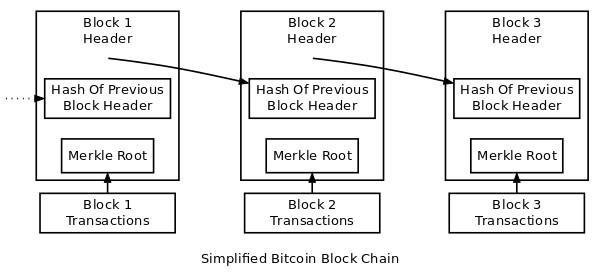
\includegraphics[width=\textwidth]{blockchain.jpg}\footnote{(http://bitcoin.stackexchange.com/questions/35448/is-it-chain-of-headers-rather-than-a-chain-of-blocks)}

Blockchains became mainly known in a financial context. The first implementation of a blockchain was used by Bitcoin, a virtual distributed crypto currency.
But in the meantime, blockchain technology has also become popular in other domains i.e. Voting-Systems \cite{yermack2017corporate} or for digital identity management \cite{isaen}. Applications that needs a high level of integrity and reliablilty could benefit from blockchains.

\imp{not finished, refs dont work?}


%\begin{itemize}
%\item What is blockchain technology?
%\item Advantages and how to use these to serve new business models?
%\item what are the well known implementations of a blockchain? (Bitcoin, Ethereum)
%\end{itemize}

\section{Ethereum}
Ethereum is a public blockchain we used for LibChain, that allows us to implement decentralized applications by means of "Smart Contracts". A smart contract is exectuable code that is stored on the blockchain. It is accessible through a unique address and triggered through transaction calls.
To execute a transaction so called gas is consumed. Gas is the fuel that is being used to pay the execution fee of the transaction\footnote{\url{http://www.reddit.com/r/ethereum/comments/2udvau/what_is_the_difference_between_gas_and_ether/}}.

The programming language to implement contracts is called \textit{Solidity}. It's a high-level turing complete programming language whose syntax is similar to JavaScript. Contracts are collections of functions and variables:

\begin{lstlisting}
contract SimpleStorage {
    uint storedData;

    function set(uint x) {
        storedData = x;
    }

    function get() constant returns (uint) {
        return storedData;
    }
}
\end{lstlisting}\footnote{\url{http://solidity.readthedocs.io/en/develop/introduction-to-smart-contracts.html}}


Mining a block on the Ethereum blockchain involves verification that exactly the deployed code was executed without tempering or inconsistencies between versions. Due to this transparency, it's easy to implement applications where normally a high level of trust between participants is needed.
    \chapter{LibChain}
LibChain allows users to create contracts between publisher and libraries that differ from the classical subscription models for digital media. 

\section{Architecture Overview}
The main architecture of LibChain is divided into three parts: React is used to implement a prototypical library page, NodeJs that provides a REST interface which enables the connection to the frontend and the Ethereum blockchain where the LibChain contracts are deployed on. Communication between the NodeJs backend and the blockchain are realised through the \texttt{Web3.js} api.

\vspace{0.3cm}
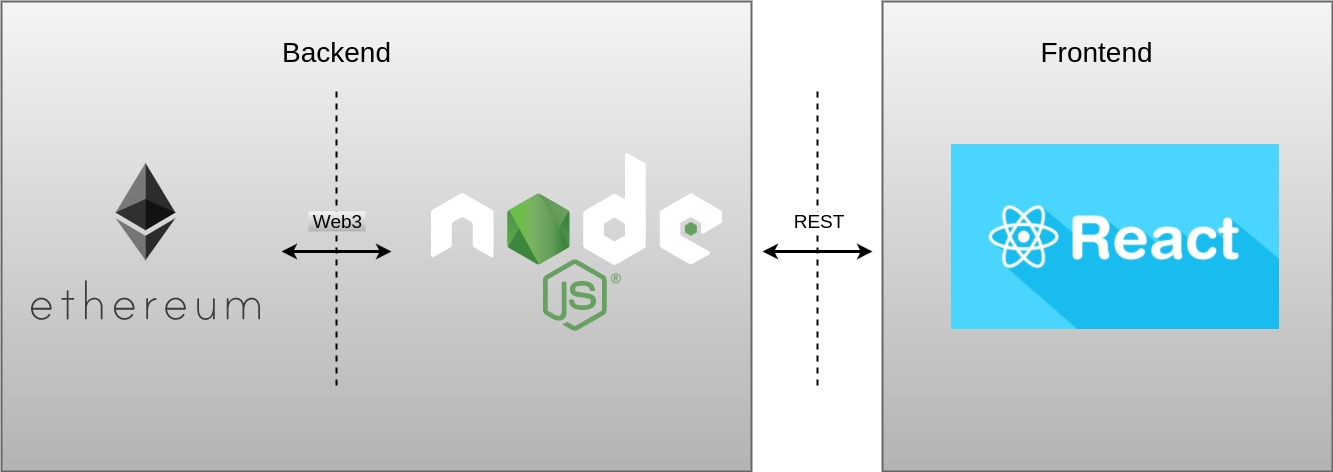
\includegraphics[width=\textwidth]{architecture.jpg}
\section{Smart Contracts}
LibChain implements smart contracts for publisher, libraries and books that provides functionality to publish, buy and lend books in the LibChain ecosystem as well as one LibChain contract that acts as a registery for all participating libraries and publishers.

\vspace{0.3cm}
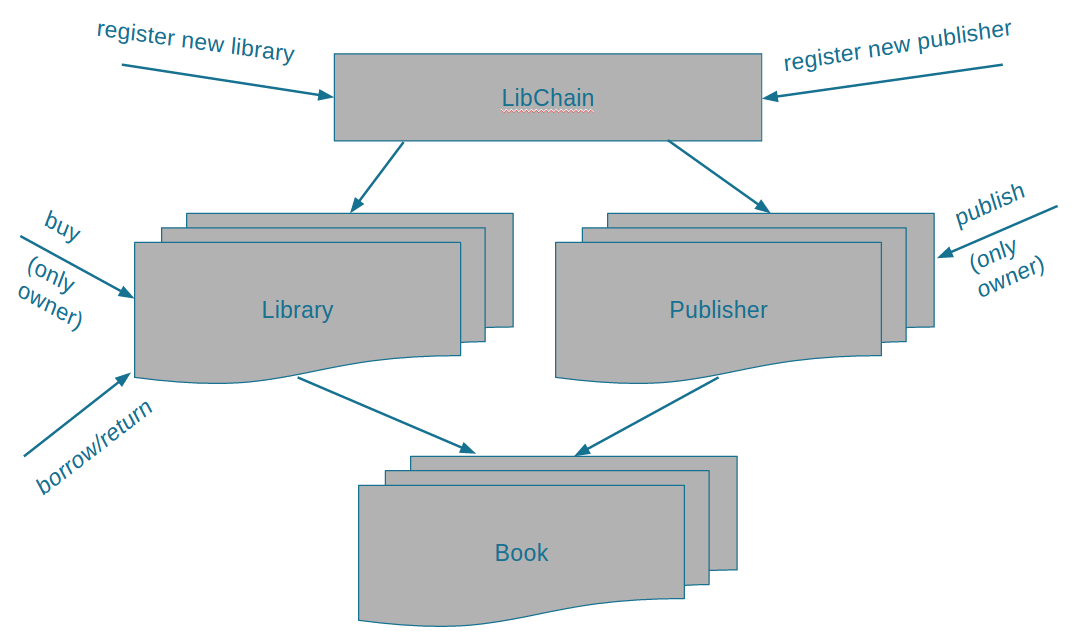
\includegraphics[width=\textwidth]{contracts.png}

\subsection{LibChain}
The LibChain contract is used to instantiate new libraries and publishers. It also provides getters for retrieving existing instances.

\subsection{Book}
The Book contract collects meta-informations like title and year of publication. It also has a field \textit{gateway} that defines the access point to the digital media (for example a link to the publishers book repository). It also contains the publisher address where an instance could be bought. Furthermore it contains some variables to get books statistics, e.g. the amount of sold instances or number of loans.


\begin{lstlisting}
contract Book {
	address public _owner;
	string public _publisher;
	uint public _year;
	string public _gateway;
	string public _isbn;

	//metrics
	uint sumOfSoldInstances;
	uint sumOfLoans;
  
	function Book(string pub, uint year, string id, string gate) {
  	_owner = msg.sender;
		_publisher = pub;
		_year = year;
		_gateway = gate;
		_isbn = id;
	}


	function getBookInfo() constant returns (uint, string, string, uint, address, address) 
	{
	 	return (_year, _isbn, _gateway, _publisher, _owner, this);
	}

	function buy(address buyer, uint amount) {
		sumOfSoldInstances++;
	}

}
\end{lstlisting}

\subsection{Publisher}
The publisher contract allows to instantiate new books and add them to the publishers catalogue. It's primarily used to publish books and sell instances to libraries.

\begin{lstlisting}
function publishBook(uint year, string id, string gate) returns(address bookContract){
		publishedBooks.push(new Book(name, year, id, gate));
		sumOfPublications++;
		(..)
		return publishedBooks[bookNum-1];
	}
\end{lstlisting}

As a book is a smart contract, it get's a unique address. Therefore, a library is able to call the \texttt{buyBook}-function to get the ownership of permanent instances.

\begin{lstlisting}
	function buyBook(address bookContract, uint amount) constant {
		Book book = Book(bookContract);
		book.buy(msg.sender, amount);	
		bills[msg.sender][bookContract] += amount;

		sumOfSoldInstances += amount;
	}
\end{lstlisting}

If an account calls the buy function, the bookaddress and the amount of instances that should be bought is associated with the buyers address. The publisher can use this information later to invoice the libraries purchase.

\begin{lstlisting}
mapping(address => mapping(address => uint)) public bills;
\end{lstlisting}

The information is mapped on the first level to the library address and on the second level to the book address.

\subsection{Library}
The library contract contains functions to buy book instances from publisher contracts and to perfom borrow and return requests.

\paragraph*{Buying books}
On a buy call, the publishers buy function is called to make a note for this purchase on the publishers site. This information could be used to pay the bill in the real world.
Then the book with the requested amount of instances is stored in the libraries inventory and makes the lending possible to the library users (see \ref{sssec:contractborrow}).

\begin{lstlisting}
	function buy(address bookContract, address publisherContract, uint amount) returns (bool) {
		Publisher pub = Publisher(publisherContract);
		pub.buyBook(bookContract, amount);
        Book book = Book(bookContract);
        if(inventory[book].amount == 0){
            inventory[book] = BookMeta(book, amount, amount);
		    _libBooks.push(book);
		} else {
            inventory[book].amount += amount;
            inventory[book].availableInstances += amount;
		}

		sumOfBoughtInstances += amount;
		return true;
	}
\end{lstlisting}


\paragraph*{Borrowing a book \label{sssec:contractborrow}}
When borrowing a book the library first performs a check whether an instance of the requested book is available or not. In addition it is ensured that a user can only borrow one instance of a book at once. 

If both these conditions are met, the users public key used for this transaction is stored in the book object in the inventory. The public key is used for checking the access authorization of the user later on(see \ref{sssec:contractaccess}).

\begin{lstlisting}
function borrow(address bookContract, string publicKey, string userId) returns (bool) {

		if(inventory[bookContract].availableInstances <= 0) return false;

		//check if this book already loaned to user
        if (sha3(users[userId].pubkeys[bookContract]) != sha3("")){
            return false;
        }


		Book book = Book(bookContract);
        for (var i = 0; i < inventory[bookContract].amount; i++) {
            if (sha3(inventory[bookContract].pubkeys[i]) == sha3("")) {
                inventory[bookContract].pubkeys[i] = publicKey;
                inventory[bookContract].availableInstances--;

                // store loan to user object
                users[userId].loanedBooks.push(bookContract);
                users[userId].pubkeys[bookContract] = publicKey;

                book.borrow(msg.sender);
                sumOfLoans++;

                return true;
            }
        }

        return false;
	}
\end{lstlisting}

\paragraph*{Access authorization \label{sssec:contractaccess}}
If a publisher receives a view-request, he can check the access authorization for this user. Here it's simply checked if a users public key is currently deposited in the book object in the library contract.
The publisher has to verify the ownership of the supplied keypair by the user with a service outside the blockchain beforehand  (see \ref{sssec:access}). 

\begin{lstlisting}
	    function hasAccessToInstance(string userId, string pubkey, address bookAddress) constant returns (uint) {
        if(sha3(pubkey) == sha3("")) return 0;

        if(sha3(users[userId].pubkeys[bookAddress]) == sha3(pubkey)){
            // has access
            return 1;
        }

        // no access
        return 0;
    }
\end{lstlisting}


\paragraph*{Return a Book}
To return a book, the public key entry of the patron for this book is deleted and the counter for availableInstances for the returned book in the inventory of the Library is increased by one again.

\begin{lstlisting}
	function returnBook(address bookContract, string publicKey, string userId) returns (bool) {
    		if(inventory[bookContract].amount <= 0) return false;
    		Book book = Book(bookContract);
            for (var i = 0; i < inventory[bookContract].amount; i++) {
                if (sha3(inventory[bookContract].pubkeys[i]) == sha3(publicKey)) {
                    inventory[bookContract].pubkeys[i] = "";
                    inventory[bookContract].availableInstances++;


                    // remove book from user object
                    for (var j = 0; j < users[userId].loanedBooks.length; j++) {
                        if(users[userId].loanedBooks[i] == bookContract){
                            delete users[userId].loanedBooks[j];
                            break;
                        }
                    }
                    users[userId].pubkeys[bookContract] = "";
                    sumOfReturns;
                    return true;
                }
            }

        return false;
    }
\end{lstlisting}

\section{Use Cases}
These use cases should demonstrate how to use the contract functions and how LibChain should be integrated in existing services of libraries and publishers.

\subsection{Book-Purchase}
\vspace{0.3cm}
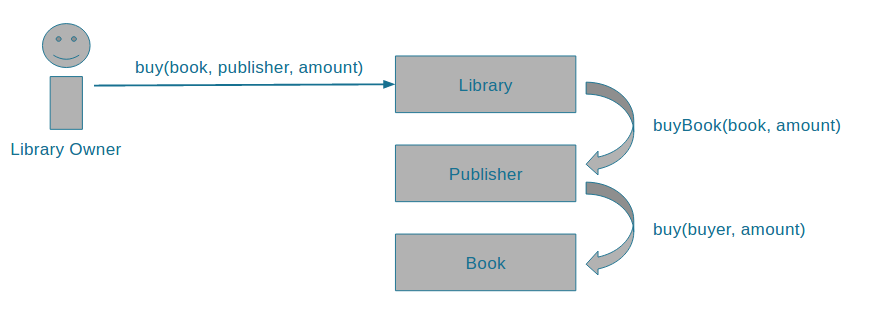
\includegraphics[width=\textwidth]{purchase.png}
\subsection{Book-Borrow}
To borrow a book, the user has to authenticate toward the library service on a classical way (e.g. username/password). The library therefore knows, that the user is authorized to borrow books. If the user wants to borrow a book, he has to create a RSA-keypair. The private key is stored on the client site whereas the public key is submitted together with the book id to the library service.
Since the user is already authenticated, the library can forward this request to the library contract without any further verification.
The contract checks the availability of the requested book instances and stores the public key (see \ref{sssec:contractborrow}) to the contract storage.

\vspace{0.3cm}
\begin{center}
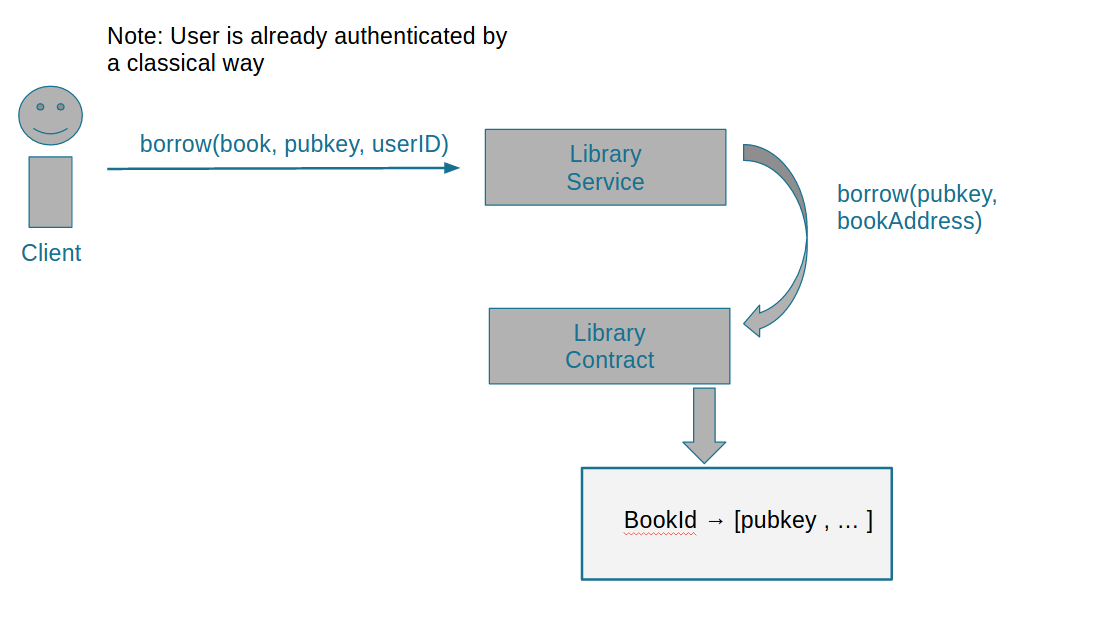
\includegraphics[width=0.7\textwidth]{borrow.png}
\end{center}

\subsection{Access to digital media \label{sssec:access}}
If a user has borrowed a book, he can call the gateway-address that is stored in the book contract. That could be a normal internet address that routes the user to the publishers book service. This enabled the publisher to implement his own level of DRM from a proprietary viewer solution to a simple pdf download.
The user can now create a view request by submitting the publickey (which he has submitted to the library on the borrow request) and the book id that he encrypts with the appropriate private key to prove his identity.

By decrypting the book id and the associated nonce with the submitted public key, the publisher can verify that the user is in possession of the private key. If this is successful, he can check that the public key is associated with a current loan of the book in the library.


\vspace{0.3cm}
\begin{center}
\includegraphics[width=0.7\textwidth]{access.png}
\end{center}

\section{Metrics}

\section{How to implement a Publisher Service?}
In order to implement a publishing service several functions in the Ethereum Smart Contract \textit{Publisher} have to be called. \\
An instance of the Publisher contract is created by calling the \\
 \verb|function newPublisher(string name, string location)| of the LibChain contract. This will return an address that represents the newly created Publisher and can be used further to instantiate the Publisher. Since the LibChain contract holds a record of all registered Publishers other Libraries can now discover the newly created Publisher at any time. Additionally they can listen to the \\
 \verb|event NewPublisher(address newPublisher| to be notified of new Publishers.
\subsection{Publishing a Book}
A potential publisher can call the\\ 
 \verb|function publishBook(uint year, string id, string gate)| of their own Publisher contract. This will return an address of a new Book contract and will also trigger the 
 \verb|event PublishBook(address newBook)|
\subsection{Selling a book}
Libraries that buy books from the Publisher will call the \\
\verb|function buyBook(address bookContract, uint amount)|  in this function there is a mapping from library address (the buyer) to yet another mapping which is from book address to amount. This is essentially the mapping relevant for accounting. By calling the associated getter an invoice can be created for each library and each book respectively.\\
 \verb|function getBill(address library_, address book_) constant returns (uint)|
\subsection{Access control}


\section{Problems and Limitations}
\begin{itemize}
\item \textbf{"out of gas" - problems}\\
Instantiations of contracts and calls of functions have to be fueled with gas. During our implementation phase, we recognised that contracts needed to remain simple and lightweight. 
For example: On our first approach, we tried to implement metrics mapped by date attributes (year and month). For this it would be necessary to do calculations on a unix timestamp to determine this data.
But we rejected this idea, because the gas usage to call these functions was extremely high. Furthermore the Ethereum documentation on this topic is fairly poor and the execution of more complex contracts seems to be premature for the technology.

\item \textbf{long function call times}\\
The call of functions, no matter if constant (calling the function wont result in a change of state) or not, needs considerable time to respond due to the block verification delays. It seems not feasible to use getters for displaying informations in the users frontend.
For our prototype of a library page, we used getters from the Library contract and the Book contract to list the book inventory in the frontend for demonstration purposes. Though we only used (constant) getter functions, the response for circa ten book entries took more then fifteen seconds. For production systems, we recommend to mirror those information on a local database and only use the blockchain methods for data modifying transactions like borrow, return or buy requests.

\item \textbf{unknown gas usage on function calls}\\
Every non constant function call has to be paid with gas. But it is hard to say how much gas is needed by a transaction in advance. A possibility could be calculating this by means of the documentation of ethereum \cite{wood2014ethereum}. But this is very low level and not really practicable. 

\item \textbf{mapping and array limitations}\\
Data managment in contracts could be very cumbersome. The usual feature to iterate through a hashmap, that we know from common programming languages is not possible with solidity.

To store user publickeys for borrowed books, we implemented following workaround:

\begin{minipage}{\linewidth}
\begin{lstlisting}

	struct BookMeta {
		Book book;
		uint amount;  // == maxIndex-1
		uint availableInstances;
		mapping(uint => string) pubkeys; //index mapping to key
	}

	mapping(address => BookMeta) public inventory;
\end{lstlisting}
\end{minipage}

The amount of books represents the upper bound of the public key mapping. To store and retrieve public keys, we used the indices as key values of the mapping.
(Note: It is also not possible to store variable sized data like strings to an array. Therefore the use of a mapping is obligatory here.)
\end{itemize}


\section{Future Work}
We implemented a base prototype of LibChain, but there a some ideas we collected for the future:

\begin{itemize}
\item \textbf{Overflow lending}\\
With LibChain we wanted to allow fairer and more accurate pricing models for publisher and library services. Currently it is possible for libraries to buy book instances similar to the puchase of books in the real world and sharing these resources with other LibChain libraries already provides a huge benefit but It would also be nice to have book access on demand. In this case, a library could lend a higher amount of instances of a book than it actually owns for a limited time and has not to buy it outright from the publisher but could pay a surge/overflow charge to the publisher instead. This would represent an attractive hybrid of the current subscription model for digital media and the pricing model for physical books at the moment.

\item \textbf{Ether-Payments}\\
In the current version, the libraries and publishers buy functions is without any limitations. Though it is guaranteed that the publisher can create valid invoices it would be desirable to implement payments directly through the contract itself by utilising the Ethereum crypto currency.

\item \textbf{Direct user access to the blockchain}\\
Library services currently have exclusive access to the data modifying functions on their contracts. They are acting for the user to execute borrow and return requests. The andvantage of this approach is, that users don't need to use the blockchain directly and old workflows and authentication systems of libraries can nearly remain unchanged.
In an enhanced LibChain implementation, it could be possible that user acting with their own Ethereum accounts on the blockchain without a direct intervention of the library service. The main function of the library would then to provide enough instances of books in the contract.

\end{itemize}

 % * overflow lending 
 % * credit for library accounts --> payments  for purchases 		with ether
 % * user access directly on the blockchain -> without library 
%    \input{./chapters/chapter3}
%    \chapter{Lessons Learned}
\section{Problems and Limitations}
\section{Future Work}
%    \input{./chapters/chapter5}
%    \input{./chapters/chapter7}

% ---------------------------------------------------------------
\backmatter % no page numbering from here
%    \addchap{Liste der Akronyme}

\begin{tabbing}
spacespacespace \= space \kill
API	 \> 	Application Programming Interface \\
ORM	 \> 	Object Relational Mapper \\
OWA	 \> 	Open Web Analytics	 \\
\end{tabbing}
\endinput

		
		% if you want to provide a glossary with explanations of important terms put it in here

\bibliographystyle{abbrvdin}
\bibliography{./bib/references}

    %\renewcommand{\thesection}{\Alph{section}}
    %\addchap{Annex}

\begin{appendix}

\section{Smart Contracts \label{annex:SmartContracts}}

\lstset{language=java,numbers=left,breaklines=true,captionpos=b,showstringspaces=false,
basicstyle={\fontfamily{pcr}\selectfont\footnotesize}}
\begin{lstlisting}
    public boolean template() {
        return true;
    }

\end{lstlisting}



\end{appendix}

\endinput


\end{document}
